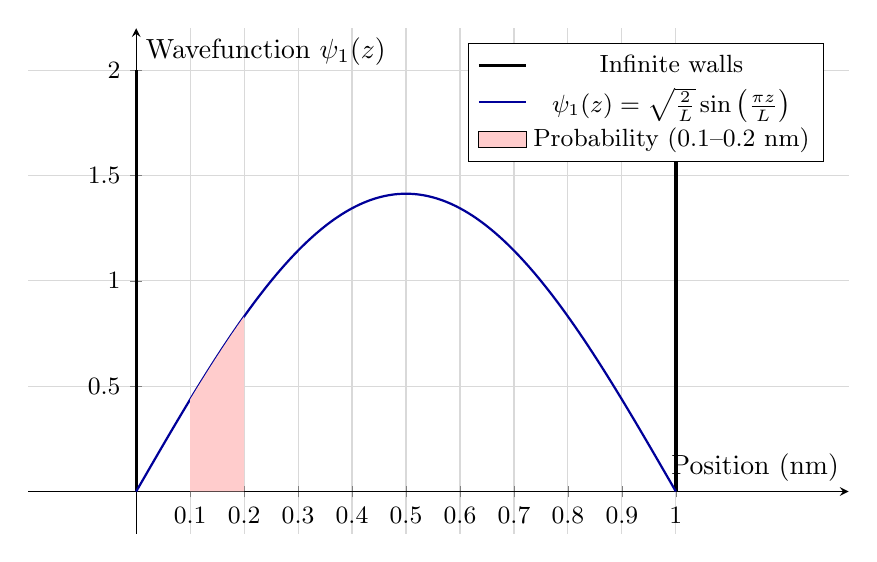
\begin{tikzpicture}
  \begin{axis}[
      xlabel={Position (nm)},
      ylabel={Wavefunction $\psi_1(z)$},
      xmin=-0.2, xmax=1.32,
      ymin=-0.2, ymax=2.2,
      grid=major,
      grid style={gray!30},
      axis lines=middle,
      width=12cm,
      height=8cm,
      xtick={0, 0.1, 0.2, 0.3, 0.4, 0.5, 0.6, 0.7, 0.8, 0.9, 1.0},
      xticklabel style={font=\small},
      yticklabel style={font=\small},
      legend pos=north east,
      legend style={font=\small}
    ]
    % Infinite potential walls (vertical lines)
    \addplot[black, very thick, domain=-0.2:2, samples=2] {-1}; %
    % \addlegendimage{black, very thick}
    \addlegendentry{Infinite walls}
    \draw[black, very thick] (axis cs:0,0) -- (axis cs:0,2);
    \draw[black, very thick] (axis cs:1,0) -- (axis cs:1,2);

    % Ground state wavefunction psi_1(z) = A_1 * sin(pi*z/L)
    % For L = 1 nm, A_1 = sqrt(2/L) = sqrt(2) for normalization
    \addplot[
      domain=0:1,
      samples=200,
      thick,
      blue!60!black
    ] {sqrt(2)*sin(deg(pi*x))};

    % Shaded area under the curve between 0.1 and 0.2 nm
    \addplot[
      domain=0.1:0.2,
      samples=100,
      fill=red!20,
      draw=none,
      area legend
    ] {sqrt(2)*sin(deg(pi*x))} \closedcycle;

    % Add legend entries
    \addlegendentry{$\psi_1(z) =
    \sqrt{\frac{2}{L}}\sin\left(\frac{\pi z}{L}\right)$}
    \addlegendentry{Probability (0.1--0.2 nm)}

    % Add wall labels
    \node[black, above] at (axis cs:1,1.8) {\small Wall};
  \end{axis}
\end{tikzpicture}
